%!TEX root = thesis.tex
\chapter{Model implementation}\label{chap:methods}
\thispagestyle{plain}

% ==== SECTION 1 ===============================================================
\section{General concepts} % (fold)
\label{sec:general_concepts}

    \subsection{Glacier volume/area scaling} % (fold)
    \label{sub:glacier_volume_area_scaling}

        % Overview

        % Physical basis, from two independet methods, ...

        % Drawbacks
    
    % subsection glacier_volume_area_scaling (end)

    \subsection{Temperature index model} % (fold)
    \label{sub:temperature_index_model}

        In a nutshell, a glaciers annual specific surface mass balance $B$ is the difference between accumulation and over the course of a year. Hereby, accumulation refers to mass gain by snowfall, avalanches, snow drift, etc., while ablation refers to mass loss via ice melt, sublimation, calving, etc. The temperature index mass balance model used by the \vas{} model relies solely on the area average monthly solid precipitation onto the glacier surface $P_i^\text{solid}$ and the monthly mean air temperature at the glacier's terminus elevation $T_i^\text{terminus}$ as input. Hereby, the index $i$ denotes the month of the year. The mass balance equation described by \citet{Marzeion2012b} reads
        \begin{align}
            \label{eq:mass-balance}
            B = \left[\sum_{i=1}^{12}\left[
                    P_i^\text{solid}  - \mu^* \cdot \max\left(T_{i}^\text{terminus} - T_\text{melt},\ 0\right)
                \right]\right] - \beta^*.
        \end{align}
        The terminus temperature $T_{i}^\text{terminus}$ is computed by scaling the monthly average air temperature $T_i$ from the climate file reference elevation $z_\text{ref}$ to the glacier's terminus elevation $z_\text{min}$ using the temperature lapse rate $\gamma_\text{temp}$.
        \begin{align}
            T_i^\text{terminus} = T_i \cdot \gamma_\text{temp} (z_\text{min} - z_\text{ref})
        \end{align}
        The temperature at the maximum glacier elevation $T_{i}^\text{max}$ is computed analogously to terminus temperature: $T_{i}^\text{max} = T_i \cdot \gamma_\text{temp} (z_\text{max} - z_\text{ref})$, whereby $z_\text{max}$ represent the maximum glacier surface elevation. The positive melting temperature is computed as the difference between terminus temperature and temperature threshold for ice melt $T_\text{melt}$, with an obvious lower bound of \SI{0}{\celsius}. The glacier's temperature sensitivity \mustar{} relates the positive melting temperature to the actual ice loss and needs to be calibrated for each glacier (as does the potential mass balance residual \bias{}). The calibration process of these mass balance parameters is described below. %(see Section~\ref{ssub:mb-calib}).
        
        The area average monthly solid precipitation onto the glacier surface $P_i^\text{solid}$ is computed from the total precipitation $P_i$ (given by the climate file) as
        \begin{align}\label{eq:solid-precip}
            P_i^\text{solid} = P_i \cdot f_\text{solid} \cdot (1 + \gamma_\text{precip} \cdot (z_\text{mean} - z_\text{ref})).
        \end{align}
        The total climatic precipitation $P_i$ is scaled from the reference elevation of the climate file $z_\text{ref}$ to the average glacier surface elevation $z_\text{mean}$ using the precipitation lapse rate $\gamma_\text{precip}$. The precipitation lapse rate $\gamma_\text{precip}$ is given in percentage of precipitation per meters of elevation change [\si{\percent\per\meter}]. The fraction of solid precipitation $f_\text{solid}$ depends on the terminus temperature $T_i^\text{terminus}$, the temperature at the maximum glacier surface elevation $T_i^\text{max}$ and the temperature thresholds for solid and liquid precipitation, $T^\text{solid}$ and $T^\text{liquid}$, respectively. For terminus temperatures below the threshold for solid precipitation, all precipitation is solid ($T_i^\text{terminus} < T^\text{solid} \ \Rightarrow f_\text{solid} = 1$). For temperatures at the maximum glacier surface elevation above the threshold for liquid precipitation, all precipitation is liquid ($T_i^\text{max} > T^\text{liquid} \Rightarrow f_\text{solid} = 0$). For temperatures in between, the fraction of solid precipitation is interpolated linearly as $f_\text{solid} = 1 + \frac{T_{i}^\text{terminus} - T^\text{solid}}{\gamma_\text{temp}\cdot(z_\text{max} - z_\text{min})}$.
        
        Climate models generally tend to underestimate the precipitation in mountainous regions, hence the monthly precipitation amount is additionally scaled by a factor $a$. While this scaling factor is implemented in the mass balance models (as \lstinline`prcp_scaling_factor`), it is not a physical component of the  mass balance equation and hence omitted in the Equation~\ref{eq:solid-precip} above. A global mean of $a = 2.5$ is found by \citet{Giesen2012}, whereas \citet{Marzeion2012c} found a mean of 2.1 for Central Europe and Scandinavia. The sensitivity study by \citet{Marzeion2012b} shows the strongest correlation between observed and modeled mass balance for $a \approx 1.3$ and the highest skill score for $a \approx 2.5$. The variability of the modeled mass-balance is quite low for values of $a \leq 2.5$.

        The values of the above mentioned hyper parameters (temperature thresholds, lapse rates, scaling factors, ...) can be calibrated, depending on the region and the used baseline climate. For Alpine model runs with the HISTALP baseline climate the following values are recommended (set as default in OGGM) and used this work \citep{Dusch2018}: $\gamma_\text{temp} = \SI{-6.5}{\kelvin\per\kilo\meter}$, $T^\text{melt} = \SI{-1.75}{\celsius}$, $\gamma_\text{precip} = 0$, $T^\text{solid} = \SI{0.0}{\celsius}$, $T^\text{liquid} = \SI{2.0}{\celsius}$, $a = 1.75$;

        \subsubsection{Calibration of the mass balance parameters}\label{ssub:mb-calib}

            A complete and thorough description of the mass balance calibration process for this particular temperature index model can be found in \citet[Section 2.1.9, 2.1.10]{Marzeion2012b} and \citet[][Section 3.3]{Maussion2019}. The following section serves as a summary.
            
            The first step is to estimate the so called \emph{candidates} $\mu(t)$ for all glaciers with available mass balance records (254 glaciers globally, see \citet{WGMS2017}). This is done by requiring the average mass balance $\overline B(t)$ over the 31-year period centered around the year $t$ to be zero and solving for $\mu(t)$.
            \begin{align}\label{eq:mu-candidates}
                \mu(t) = \frac{P_\text{clim}^\text{solid}(t)}{\max(T_\text{clim}^\text{terminus(t)} - T_\text{melt}\, 0)},
            \end{align}
            whereby $P_{\text{clim}}^{\text{solid}}(t)$ and $T_{\text{clim}}^{\text{terminus}}(t)$ are the average yearly solid precipitation amount and average yearly air temperature at the glaciers terminus during the climatological period centered around the year $t$, respectively. The next step is to solve the mass balance equation (Eq.~\ref{eq:mass-balance}) for each candidate $\mu(t)$ and compare it to the mass balance observations. The computed difference $\beta(t)$ is a measure of how good the temperature sensitivity candidate $\mu(t)$ approximates the \textit{real} value of \mustar{}. Hence, \mustar{} is chosen as the candidate $\mu(t = t^*)$ for which the absolute bias is minimal $\beta^* \coloneqq \beta(t = t^*) \approx 0$, which in the best case is around zero. Hereby, the \textit{equilibrium year} \tstar{} represents the center of a 31-year climatic period where the given glacier geometry would stay in equilibrium. However, this is more of a model parameter and should not be overinterpreted as a real live value. The same is true for the corresponding temperature sensitivity \mustar{} and mass balance residual \bias{}.

            For all glaciers without mass balance records, \tstar{} and \bias{} are interpolated from the ten closest glaciers, inversely weighted with distance. The temperature sensitivity is computed by requiring the mass balance to be zero $\overline B(t^*) = 0$ and solving for \mustar{}. The temperature sensitivity \mustar{} depends highly on glacier specific factors, such as avalanches from surrounding terrain, topographical shading, etc. Therefore, \mustar{} can vary drastically from one glacier to another, even between neighboring glaciers. On the other hand, it is intuitively more likely for a glacier to be in equilibrium if its surrounding glaciers are in equilibrium as well. This is one major factor, why the interpolation of \tstar{} instead of \mustar{} reduces the mass balance error in a leave--one--out cross--validation \citep[cf.][]{Marzeion2012b, Maussion2019}.


        \subsubsection{Implementation note} % (fold)
        \label{ssub:mb_calib_implementation_note}

            The results of the steps above depend on the glacier outlines, the climate data and the mass balance hyper parameters (i.e., the temperature thresholds, lapse rates and the precipitation scaling factor). The equilibrium year \tstar{} and mass balance residual \bias{} computed for each reference glacier is stored in the \lstinline`ref_tstars.csv` file. Hence, for a given combination of RGI version, climate data and hyper parameters the calibration for the reference glaciers has to be done only once. Afterwards, it can be read directly from the corresponding file. OGGM comes with reference tables for combinations of RGI v5 and v6 and CRU4 and HISTALP.
        
        % subsubsection mb_calib_implementation_note (end) 

        \subsubsection{Differences between the flowline mass balance model and the \vas{} mass balance model}

            The \vas{} mass balance model computes an average mass balance value for the entire glacier. The mass balance model requires only the minimal and maximal glacier elevation as additional input parameters ($z_\text{min}$, $z_\text{max}$), to compute the monthly terminus temperature $T_i^\text{termiuns}$ and the area averaged monthly amount of solid precipitation $P_i^\text{solid}$. The flowline model, on the other hand, requires a mass balance value for each grid point of the flowline (i.e., for each elevation band). Therefore, the mass balance is a function of elevation $B(z)$ and the elevation of the grid points must be supplied. Solid precipitation and air temperature are then computed for the given points of elevation, resulting in a point mass balance.
    
    % subsection temperature_index_model (end)

    \subsection{Glacier evolution model} % (fold)
    \label{sub:glacier_evolution_model}

        % Volume/area scaling must be used in conjuncture with proper response time scaling (Bahr, 2015)
        \Vas{} is derived from the full set of continuum equations with no assumptions of plane strain, shallow ice, perfect plasticity, or steady state conditions. This derivation from the fully time dependent equation of motion allows the volume $V$, area $A$ and scaling constant $c_A$ to change with time. Especially the scaling constant $c_A$ can incorporate transient behavior, since it depends on closing conditions which show an explicit time dependency. However, to explicitly include a temporal component, \vas{} has to be used in conjuncture with proper response time scaling. Response time scaling is a separate but equally valid scaling relation, derived during the same dimensionless analysis. Hence, these two scaling relations cannot be separated and have to be applied together to successfully model glacier evolution \citep{Bahr2015}.

        % Initialization: start with area, compute volume and length from scaling relations
        The \vas{} model starts with an initial glacier surface area $A_0$ as input. The initial glacier volume $V_0$ and the initial glacier length $L_0$ are computed using the \vas{} relation and the inverted volume/length scaling relation, respectively (cf. Section~\ref{sub:glacier_volume_area_scaling}).
        \begin{align}
            \begin{split}
                V_0 = c_A\cdot A_0^\gamma \qquad\qquad L_0 = \left(\frac{V_0}{c_L}\right)^\frac{1}{q}
            \end{split}
        \end{align}
        Additionally, only a mass balance model and the initial terminus elevation $z_{\text{min},0}$ and maximal glacier surface elevation $z_\text{max}$ are needed.

        % Yearly steps
        The \vas{} model runs with yearly time steps $\Delta t = \SI{1}{\year}$. Each time step from year $t$ to year $t+1$ includes the following steps:
        \begin{enumerate}
            \item Compute the time scale of the glacier's length change response to volume change $\tau_L$ and the time scale of the glacier's surface area change response to volume change $\tau_A$ as
            \begin{align}
                \begin{split}
                    \tau_L(t) = \frac{V(t)}{P^\text{solid}_\text{clim}(t^*)\cdot A(t)}
                    \qquad\qquad
                    \tau_A(t) = \tau_L(t)\frac{A(t)}{L(t)^2}
                \end{split}
            \end{align}
            As introduced during the calibration process, $P^\text{solid}_\text{clim}(t^*)$ is the average solid precipitation during the 31-year period centered around \tstar{}. For more details see \citet{Marzeion2012b}. The implementation includes lower bounds for both time scales as well as the climatological turnover, for details see Section~\ref{sub:glacier_evolution_model_implementation}.
            \item Get the specific mass balance $B(t)$ from mass balance model, by solving Equation~\ref{eq:mass-balance}. For implementation details see Section~\ref{sub:mass_balance_models_implementation}
            \item Compute the volume change $\Delta V(t) = \frac{1}{\rho_\text{ice}}A(t)\cdot B(t)$ as product of specific mass balance and glacier surface area. The volume change happens instantaneously, i.e., over one time step, hence the updated volume equals the sum of current volume and volume change $V(t+1) = V(t) + \Delta V(t)$.
            \item The (hypothetical) equilibrium surface area can be computed by inverting the \vas{} relation $(V(t+1)/c_A)^{1/\gamma}$. However, the surface area does not change instantaneously, and proper response time scaling must be applied. Hence, the area change is computed as
            \begin{align}
                \Delta A(t) = \frac{1}{\tau_A}\left(\left(\frac{V(t+1)}{c_A}\right)^\frac{1}{\gamma} - A(t)\right).
            \end{align}
            The updated area then equals the sum of current area and area change $A(t+1) = A(t) + \Delta A(t)$.
            \item The updated glacier length and length change are computed analogously to the glacier surface elevation. $L(t+1) = L(t) + \Delta L(t)$, with
            \begin{align}
                \Delta L(t) = \frac{1}{\tau_L}\left(\left(\frac{V(t+1)}{c_L}\right)^\frac{1}{q} - L(t)\right).
            \end{align}
            \item Adjust terminus elevation $z_\text{min}$, assuming a linear elevation change with changing glacier length (i.e., constant slope):
            \begin{align}
                z_\text{min}(t+1) = z_\text{max} + \frac{L(t)}{L_0}(z_{\text{min},0} - z_\text{max})
            \end{align}
            The maximum glacier elevation stays constant during the entire model run $z_\text{max} = \text{const.}$
            
        \end{enumerate}
        
        \begin{figure}[tbh]
            \centering
            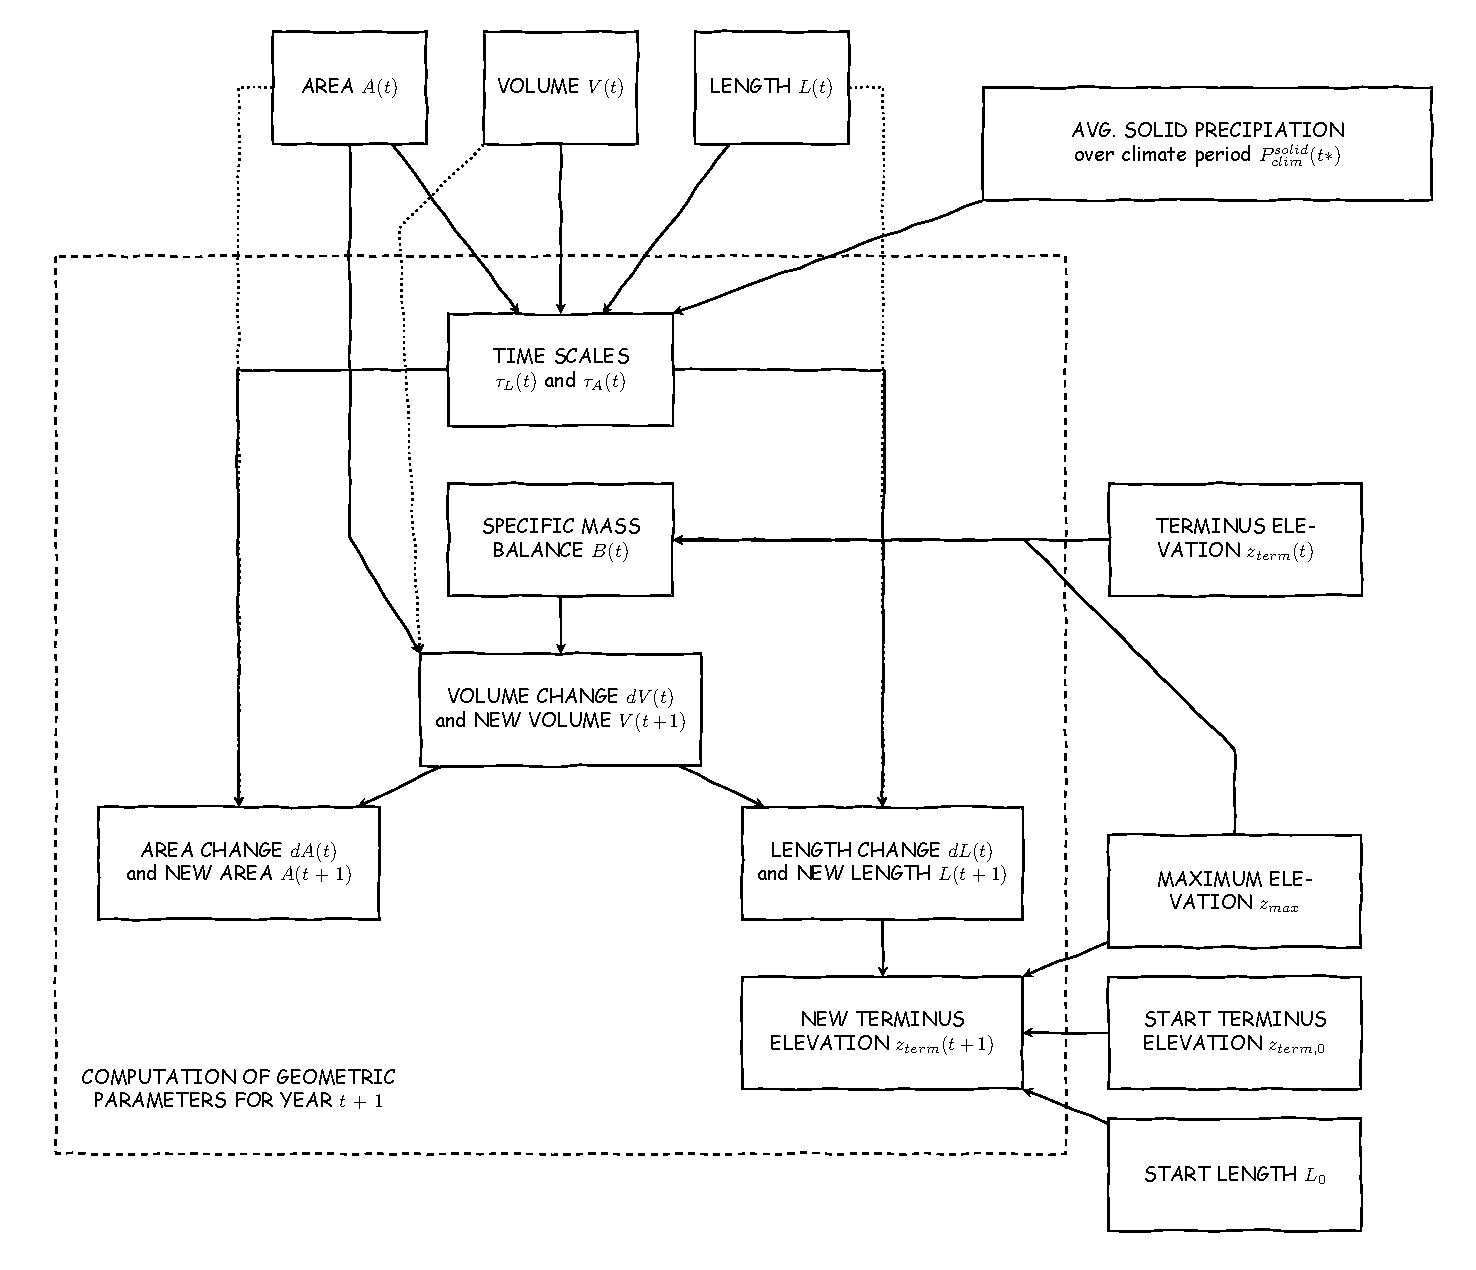
\includegraphics[width=\textwidth]{../flowchart/iterations/scaling.pdf}
            \caption{Schematic of the glacier evolution model's time stepping.}
            \label{fig:iteration-scheme}
        \end{figure}
        
        % Start area finding process ???
    
    % subsection glacier_evolution_model (end)

% section general_concepts (end)

% ==== SECTION 2 ===============================================================
\section{Implementation} % (fold)
\label{sec:implementation}

    \subsection{Mass balance models} % (fold)
    \label{sub:mass_balance_models_implementation}

        \subsubsection{Volume/area scaling mass balance model} % (fold)
        \label{ssub:volume_area_scaling_mass_balance_model_implementation}

            The \lstinline`VAScalingMassBalance` model is the implementation of the \textit{original} mass balance model by \citet{Marzeion2012b}. The model computes the mass balance of a glacier during the climate data period. The general concept is fairly similar to the \lstinline`oggm.core.massbalance.PastMassBalance` model. The main difference is, that the \vas{} mass balance model returns only one glacier wide average mass balance value, instead of point mass balance values for the different elevation bands.

            The mass balance model is initialized for a single glacier, denoted by the OGGM specific glacier directory \lstinline`gdir`. Per default, the model will use the calibrated mass balance parameters \mustar{} and \bias{} and read temperature and precipitation records from the preprocessed climate file \lstinline`climate_historical`. An alternative climate file can be used, by supplying either the filename and/or it's suffix via the parameters \lstinline`filename` and \lstinline`input_filesuffix`, repecitvely. It is possible to specify the start year and end year of the climate period (\lstinline`ys` and \lstinline`ye`), if not all available data should be used. The parameter \lstinline`repeat` controlls whether the climate period given by \lstinline`[ys, ye]` should be repeated indefinitely in a circular way.

            The \vas{} mass balance model inherits the following methods from the \lstinline`oggm.core.massbalance.MassBalanceModel` super class:
            \begin{itemize}
                \item \lstinline`get_annual_climate()` and \lstinline`get_monthly_climate()` compute and return the mass balance relevant climate information, i.e. positive air temperature at the terminus elevation in \si{\celsius} and solid precipitation amount in \si{\kg\per\square\m}, for the given year and month/year combination, respectively.
                \item \lstinline`get_annual_mb()` and \lstinline`get_monthly_mb()` compute and return the glacier wide average mass balance in \si{\m\per\s}, for the given year and month/year combination, respectively. The possible mass balance residual \bias{} is applied.
                \item \lstinline`get_specific_mb()` and \lstinline`get_monthly_specific_mb()` compute and return the glacier wide average specific mass balance in \si{mm w.e.\per yr}, for the given year and month/year combination, respectively. The possible mass balance residual \bias{} is applied.
            \end{itemize}
            All methods need the glacier terminus elevation \lstinline`min_hgt` and the maximal glacier surface elevation \lstinline`max_hgt` as parameters. The date is supplied via the \lstinline`year` parameter, using the hydrological float year convention. Given that the scaling mass balance model computes the glacier wide average mass balance, it is not possible to estimate the equilibrium line altitude. Hence, the the method \lstinline`get_ela()` is not implemented, in contrast to the \lstinline`PastMassBalance` model.
        
        % subsubsection volume_area_scaling_mass_balance_model_implementation (end)

        \subsubsection{Constant climate scenario} % (fold)
        \label{ssub:constant_climate_scenario_implementation}
            The \lstinline`ConstantMassBalance` model simulates a constant climate based on the observations averaged over a 31-year period centered on a given year \lstinline`y0`. Hence, the specific mass balance does not change from year to year. The task \lstinline`run_constant_climate(gdir, ...)` initializes a \lstinline`ConstantMassBalance` for the given glacier \lstinline`gdir` and runs for a given number of years \lstinline`nyears`. The task takes an additional temperature bias as parameters \lstinline`temp_bias`, to alter the observed climate records.

            The same idea of a constant climate is used during the mass balance calibration, solving the mass balance equation (Equation~\ref{eq:mass-balance}) for the temperature sensitivity \mustar. So per definition, \mustar{} is the temperature sensitivity to keep the glacier in equilibrium over the 31-year climate period centered around the \textit{equilibrium year} \tstar{} while neglecting a potential mass balance residual \bias. Consequentially, a \lstinline`ConstantMassBalance` model with \lstinline`y0` = \tstar{} keeps the glacier in equilibrium.
        
        % subsubsection constant_climate_scenario_implementation (end)

        \subsubsection{Random climate scenario} % (fold)
        \label{ssub:random_climate_scenario_implementation}

            Similar to the \lstinline`ConstantMassBalance` model, the \lstinline`RandomMassBalance` model is based on a 31-year period centered on a given year `y0`. However, the mass balance years are randomly shuffeled within that period. More precise, for each simulated year the model computes the specific mass balance using temperature and precipitation records from a randomly selected year within the given period. Hence, the model runs on a synthetic random climate scenario based on actual observations. A seed \lstinline`seed`' for the random generatore can be supplied as parameter, to allow for reproducibility. Additionally, it is possible to choose between draws with and without replacement via the \lstinline`unique_sample` parameter.

            The task \lstinline`run_random_climate(gdir, ...)` works analogously to the task \lstinline`run_constant_climate(gdir, ...)`, using an instance of \lstinline`RandomMassBalance` model instead of the \lstinline`ConstantMassBalance` model. Hence, using the climatological period centered around \lstinline`y0` = \tstar, the model glacier should stay in an equilibrium state while underlying minor fluctuations. Supplying a positive or negative temperature bias will result in a retreating or advancing model glacier, respectively, reaching a new equilibrium after some years.
        
        % subsubsection random_climate_scenario_implementation (end)
    
    % subsection mass_balance_models_implementation (end)

    \subsection{Glacier evolution model} % (fold)
    \label{sub:glacier_evolution_model_implementation}

        The \lstinline`oggm-vas.VAScalingModel` is the implementation of the above describe glacier evolution model (see Section~\ref{sub:glacier_evolution_model}, \citet[cf.]{Marzeion2012b}) into the OGGM framework. The full source code is publicly available on \href{https://github.com/OGGM/oggm-vas}{GitHub}.

        An instance of the \lstinline`oggm-vas.VAScalingModel` class is initialized with the initial area \lstinline`area_m2_0`, the initial glacier terminus elevation \lstinline`min_hgt` and maximum glacier surface elevation \lstinline`max_hgt` and an instance of a \lstinline`oggm-vas.VAScalingMassBalance` model. Additionally, the start year of the simulation \lstinline`year_0` must be defined. Those initial values are stored as instance variables, since they are needed for later computations. Other than that, the \lstinline`oggm-vas.VAScalingModel` object stores all model parameters as instance variables for the current year it is in. This includes glacier geometries ($V$, $A$, $L$, $z_\text{min}$, $z_\text{max}$) and their changes ($\Delta V$, $\Delta A$, $\Delta L$), time scales ($\tau_A$, $\tau_L$), the mass balance model and the specific mass balance $B$, but also constants like the scaling parameters ($c_A$, $\gamma$, $c_L$, $q$) and ice density $\rho_\text{ice}$.

        To advance the glacier model, there are three different methods. The \lstinline`step()` method advances the model by one year, following the above described steps (see Section~\ref{sub:glacier_evolution_model}). The method \lstinline`run_until(year_end)` runs the model until the specified year and returns the geometric glacier parameters at the end of the model evolution (year, length, area, volume, terminus elevation and specific mass balance). Thereby, the model starts from whatever year it currently is in. It is possible to start the model run from \lstinline`year_0` with the flag \lstinline`reset`. The method \lstinline`run_until_and_store()` works analagous to the previous one, with the difference that all parameters are stored for each time step (i.e., for each year). The resulting data set is returned and possible stored to file, if a file path is give. The method \lstinline`run_until_equilibrium()` tries to run the glacier model until an equilibirum state is reached. The model runs for a fixed number of iteratrions \lstinline`max_ite`, the total elapsed time changes with the chosen time step \lstinline`ystep`. The iteration breaks, either if the glacier volume is below \SI{1}{\cubic\meter} or an equilibirum is reached. An equilibrium state is reached, if the volume change rate $|V(t) - V(t+\Delta t)|/V(t)$ falls below a given value \lstinline`rate`. Therefore, the method can only be used with a constant climate scenario (see Section~\ref{ssub:constant_climate_scenario_implementation}).
    
    % subsection glacier_evolution_model_implementation (end)


% section implementation (end)


% ==== SECTION 3 ===============================================================
\section{Experimental setup} % (fold)
\label{sec:experimental_setup}

    \subsection{Equilibrium experiments} % (fold)
    \label{sub:equilibrium_experiments_setup}
        As most things in nature, glaciers strive toward an equilibrium condition by reacting to changes in climate with changes in geometry. Subjecting a glacier model to a constant climate (or a step change in climate) is a useful tool to asses the behavior of glacier models. Analyzing the behavior of glacier models subjected to a step change in climatic conditions is a widely used practice to estimate response times and get an insight into the dynamics of a numerical model. The OGGM provides two convenient mass balance models (or rather climate scenarios) for such equilibrium experiment: the \lstinline`ConstantMassBalance` model and the \lstinline`RandomMassBalance` model. The implementation and workings of both mass balance models are described in Section~\ref{ssub:constant_climate_scenario_implementation} and Section~\ref{ssub:random_climate_scenario_implementation}, respectively.

        The equilibrium experiments are performed on all alpine glaciers and using the HISTALP dataset \citep{Auer2007} as climate input data, with the corresponding hyper parameters (see \href{https://oggm.org/2018/08/10/histalp-parameters/}{Mass-balance model calibration for the Alps} on the OGGM blog for more information).

        The needed preprocessing includes GIS tasks (computing a local grid using the Shuttle Radar Topography Mission (\href{http://srtm.csi.cgiar.org/}{SRTM}, \citet{Jarvis2008}) digital elevation model (DEM) and the outline from the Randolph Glacier Inventory \citep{RGI2017,Pfeffer2014}; computing centerlines), climate tasks (preparing the HISTALP data), mass balance calibration (computing the temperature sensitivity \mustar{}) as well as the inversion tasks (estimating a bed topography) for the flowline model. For more details about the OGGM workflow see \citep{Maussion2019} and the \href{https://docs.oggm.org}{OGGM documentation}.

        As explained above, the mass balance model calibration depends on the chosen \textit{equilibrium year} \tstar{}. Hence, if both evolution models are supposed to run under the exact same climatic conditions (i.e., using the same temperature and precipitation records from the same 31-year period), \tstar{} must be same for both evolution models. This is done by computing the temperature sensitivity \mustar{} for both models using the same \tstar{} reference table \lstinline`oggm_ref_tstars_rgi6_histalp.csv`. (cf. Section~\ref{ssub:mb-calib}) and no mass balance residual ($\beta^*$ = 0). For the regional run, however, each glacier uses it's own ``best fitting'' \tstar{} and therefore \mustar. The calibration of the \mustar{} parameter is based on \citet{Marzeion2012b}, ensuring a minimal mass balance error due to the spatial interpolation of \tstar{} rather than \mustar{} \citep[for more details see][Sec. 3.3]{Maussion2019}.

        Both evolution models run for 1'000 years with the \lstinline`ConstantMassBalance` model and for 10'000 years with the \lstinline`RandomMassBalance` model. Both mass balance models are initialized around the respective \textit{equilibrium year} for each glacier, \lstinline`y0` = \tstar. Furthermore, each climate scenario runs with three different temperature biases of \SI{0}{\celsius}, \SI{-0.5}{\celsius} and \SI{+0.5}{\celsius} resulting in an equilibrium run, a run with positive and negative mass balance bias, respectively. The yearly geometric properties (length, area and volume) of the model glacier are stored to allow further investigations. In addition to the absolute values, a dataset with normalized values (with respect to the initial value) is produced, allowing better comparability.

        
        \subsubsection{Single glacier under random climate scenario} % (fold)
        \label{ssub:single_glacier_under_random_climate_scenario}
            

            As explained above, the mass balance model calibration as well as the random mass balance model depend on the chosen \textit{equilibrium year} \tstar{}. Hence, if both evolution models are supposed to run under the exact same climatic conditions (i.e., using the same temperature and precipitation records from the same 31-year period), \tstar{} must be same for both evolution models. This is done by computing the temperature sensitivity \mustar{} for both models using the same \tstar{} reference table \lstinline`oggm_ref_tstars_rgi6_histalp.csv`. (cf. Section~\ref{ssub:mb-calib}). The mass balance residual is omitted ($\beta^*$ = 0) during the model run, keep the glacier in equilibrium.

        Both evolution models run for 1'000 years with the \lstinline`ConstantMassBalance` model and for 10'000 years with the \lstinline`RandomMassBalance` model. Both mass balance models are initialized around the respective \textit{equilibrium year} for each glacier, \lstinline`y0` = \tstar. Furthermore, each climate scenario runs with three different temperature biases of \SI{0}{\celsius}, \SI{-0.5}{\celsius} and \SI{+0.5}{\celsius} resulting in an equilibrium run, a run with positive and negative mass balance bias, respectively. The yearly geometric properties (length, area and volume) of the model glacier are stored to allow further investigations. In addition to the absolute values, a dataset with normalized values (with respect to the initial value) is produced, allowing better comparability.
        % subsubsection single_glacier_under_random_climate_scenario (end)


        \subsubsection{Autocorrelation analysis} % (fold)
        \label{ssub:autocorrelation_analysis_setup}

            
        
        % subsubsection autocorrelation_analysis_setup (end)

    % subsection equilibrium_experiments (end)

% section experimental_setup (end)